\pdfbookmark{\tth Application}{ttH_dilep application}
\chapter{\tth Application}
\label{Application}

The CERN computational resources, the Worldwide LHC Computing Grid, are organized in a hierarchy divided in 4 tiers. Each tier is made by one or more computing centers and each tier has a set of specific tasks and services to perform. The objective of the whole grid is to store, filter and analyse all the data gathered at the LHC.

The Tier-0 is the data center located at CERN. It provides 20\% of the total grid computing capacity, and its objective is to store and reconstruct the raw data gathered at the detectors in the LHC into meaningful information, usable by the remaining tiers. This tier distributes the raw data and the reconstructed output by the 11 Tier-1 computational centers, spread among the different countries that are part of CERN.

Tier-1 computational centers are responsible for storing a portion of the raw and reconstructed data and provide support to the grid 24/7. In this tier, the reconstructed data suffers more reprocessing, in order to refine it by filtering only relevante information and reducing the size of the data that is then transferred to the Tier-2 computational centers. This tier also stores the outputs of the simulations performed at Tier-2. The Tier-0 center is connected to the 11 Tier-1 centers by high bandwidth optical fiber links, which consists of the LHC Optical Private Network.

There are around 140 Tier-2 computational centers around the world. Their main purpose is to perform Monte-Carlo simulations with the data received from the Tier-1 centers, but also perform a portion of the events reconstructions. The Tier-3 centers range from university clusters to small personnal computers, and they perform most of the events reconstruction and final data analysis.

The LIP research group developed the \tth application to solve the problem presented in section \ref{Motivation}, and it fits in the Tier-3 hierarchy level of event reconstruction and analysis applications. Its name derived from the problem it was design to solve: the tt is relative to the kinematical reconstruction of the two Top Quarks, the \ttbar system, resultant from a head-on particle collision; the H is relative to the Higgs boson reconstruction; the dilep is the name of the routine responsable for the kinematical reconstruction, and it needs two leptons (di-lep) as input.

The application has two main dependencies. The first, and most important, is on the ROOT \ref{CERN:ROOT} object oriented framework, developed at CERN, only available in C++. This framework provides a set of funcionalities oriented for handling, analyzing and displaying results for large amounts of data. It has capabilities of reading and storing data in the standard formats accepted by all the tiers centers, classes for representing physics information, mathematical routines, pseudorandom number generators, histograming, curve fitting minimization and visualization methods. It was originally designed and currently developed mostly by physicists with little knowledge on computer science. This results in a framework that has much room for improvement through a code restructuration in several routines, mostly related to auxiliary functionality, rather than visualization and data storage. Some of the mathematical routines implemented could be replaced by dependencies on other much more stable and faster libraries, such as BLAS \ref{BLAS} or MKL \ref{MKL}. There is an extension to ROOT, the Parallel ROOT Facility (PROOF) \ref{CERN:PROOF}, for parallelization of the work in distributed memory systems, which is not the focus of this thesis work. There is no support nor existing routines parallelized for shared memory systems, which could be made but would require restructuration of portions of the framework code.

The second dependency is on the LipMiniAnalysis library. It is a strip-down version of LipCbrAnalysis, a library developed LIP for in-house use, which provides a skeleton for creating an analysis application. It has the functionality usually necessary in most analysis developed by LIP, and is also prepared for reading a data format different from what is provided by Tier-2, which suffers a filter of the events most likely to provide relevant information after the reconstruction. This library is also not designed for parallelization in shared and distributed memory systems.

\pdfbookmark{Application Flow}{application flow}
\section{Application Flow}
\label{Application:Flow}

This section describes the workflow of the \tth analysis. The callgrind tool from Valgrind \ref{Callgrind} was used to obtain the callgraph of the application, also providing some insight on the time that was being spent in each of its routines. Further analysis of the code itself was necessary to get a better understanding of the application behaviour. In figure \ref{fig:CallgraphOriginal} is presented the callgraph of \tth for 128 variations per combination.

\begin{figure}[!htp]
	\begin{center}
		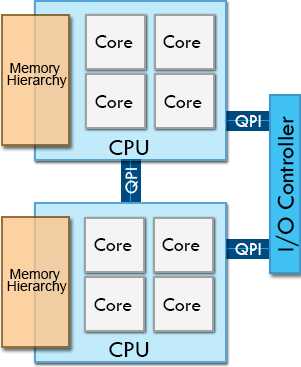
\includegraphics[scale=0.5]{../../common/img/numa_qpi.png}
		\caption{Schematic representation of a NUMA system with QPI interface.}
		\label{fig:CallgraphOriginal}
	\end{center}
\end{figure}

The \ttLoop is the main method of the application. Its purpose is to iterate through all events in the input file and perform 21 filtering and processing tasks (known as cuts) to each event. The most evident problem with the application, inherited from the LipMiniAnalysis library, is the non existence of a data structure on memory holding the events to process. Each input file has around 1 GByte that makes perfectly possible to be stored on RAM memory. However, for each event its information is read from the file and loaded to hundreds of global variables and then it is submited through the cuts. If all the events were read at once, it would be possible to take advantage of the higher bandwidth of sequential reads to the hard drive. Even the overhead of creating such data structure for the events would be compensated by the faster acesses and possibility of easier parallelization of the analysis at the event level, since the events have no dependencies between them.

Every method starting with a capital T refers to the ROOT framework. They are only being used for reading the input file and writing the results. The \ttDoCuts method performs the 21 cuts referred above. It is on cut 20 that \ttDilepKinFit is called, which becomes the most time consuming task as the number of variations per combination increases, as seen from table \ref{tab:TempoKinFit}, therefore, the efforts on improving the performance must be focused on this routine.

\begin{table}[!htp]
	\begin{center}
		\begin{tabular}{|c|c|c|c|c|c|c|c|c|c|c|c|}
			\hline
			\textbf{# of variations/combination} & 1 & 2 & 4 & 8 & 16 & 32 & 64 & 128 & 256 & 512 & 1024 \\ \hline
			\textbf{\% of time} & - & - & - & - & - & - & - & - & - & - & - \\ \hline
		\end{tabular}
		\caption{Percentage of the total execution time spent on the \ttDilepKinFit routine for various numbers of variations per combination.}
		\label{tab:TempoKinFit}
	\end{center}
\end{table}

\todo{terminar tabela com \% tempo na ttdilep}

\pdfbookmark{ttDilepKinFit Routine}{ttDilepKinFit routine}
\section{\ttDilepKinFit Routine}
\label{Application:ttDilepKinFit}



\begin{figure}[!htp]
	\begin{center}
		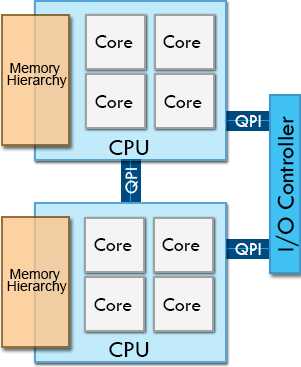
\includegraphics[scale=0.5]{../../common/img/numa_qpi.png}
		\caption{Schematic representation of a NUMA system with QPI interface.}
		\label{fig:CallgraphOriginal}
	\end{center}
\end{figure}